\chapter{MOTMaster}\label{chap:compinterface}

\section{Chapter Overview}\label{sec:compinterface_overview}
The aim of this chapter is to provide a description of the MOTMaster
software, which was developed from a pre-existing version during my PhD. The
design of MOTMaster assumes very little about the particular experiment it is
being used for, so much of the discussion in this chapter will be kept
general. This chapter begins with a motivating the need to extend MOTMaster by
developing a graphical interface to simplify the creation of experimental
sequences, as well as implementing new methods of controlling hardware. This
is followed by a description of how input and output channels are controlled using MOTMaster in~\SectionRef{sec:mm_interface}. The structure of a MOTMaster sequence, along with how it runs an experiment is then presented in~\SectionRef{sec:mm_sequences}. Finally, the specific hardware used in this experiment and an overview of each major step of the experiment is given in~\SectionRef{sec:mm_control_hardware}.

\section{Motivation}\label{sec:mm_motivation}
In the initial stages of my PhD, I decided to use Cicero Word
Generator~\cite{Keshet2012} to control the hardware for the experiment. This
is a graphical-based control system developed by Wolfgang Ketterle's group at
MIT, which was designed for controlling atomic physics experiments using
National Instruments hardware. Over time, as the experiment became more
complex, it started to become apparent that Cicero was not suited to meet all
of our requirements for control software. This was most evident in the
control of the M-Squared Raman laser system. Cicero also takes an
appreciable amount of time (around \sivalue{300}{\milli\second}) to
re-calculate the experiment sequence between each shot. Since the design of
Cicero was aimed at controlling experiments that take many seconds per cycle,
this dead time between each cycle is not significant on those time scales. In
contrast, each cycle of this experiment takes around
\sivalue{250}{\milli\second}. This unnecessary dead time needed to be
addressed if we hoped to improve the repetition rate. \par\noindent
After it became clear that a potentially large amount of work would be needed
to improve Cicero, I decided that it was worth moving to a new control
system. A collection of programs, named EDMSuite, has been developed by
people in \ac{ccm} to control a range of experiments within the group. One
application, MOTMaster, was designed to control and acquire data from
experiments investigating cold atoms trapped in a \ac{mot}. However, its method of structuring experimental sequences was
inconvenient, as it lacked an intuitive graphical user interface. During the
process of switching to using MOTMaster to control the experiment, I designed
a graphical method of structuring sequences, which functioned identically on
a device level to the original method of defining sequences. In addition to
this, I included an interface to the M Squared laser system, so that it could
be controlled using MOTMaster. A schematic of the structure of MOTMaster and how it interfaces with hardware is shown in~\FigureRef{fig:motmaster_structre}. It is designed so that experiments can be controlled without requiring specific details about the hardware in use.
\begin{figure}[!htbp]
    \centering
    \fontsize{16pt}{16pt}
    \resizebox{0.4\textwidth}{!}{\input{motmaster_structure.pdf_tex}}
    \caption[Schematic diagram of MOTMaster and hardware interface.]{Schematic diagram of MOTMaster and the hardware it controls. A sequence is built using the user interface, which then uses separate modules to communicate to the hardware. In this way, an experiment can be controlled without requiring specific knowledge of the hardware.}
    \label{fig:motmaster_structure}
\end{figure}
\section{Interfacing wth Hardware}\label{sec:mm_interface}

The majority of the experimental hardware is controlled using analogue and
digital voltages that are generated by \ac{daq} cards manufactured by
National Instruments. MOTMaster is compatible with cards that use either the
NI-DAQmx or NI-HSDIO device drivers. These are used to configure the
generation or acquisition of digital or analogue voltage waveforms. By design, they are
capable of precisely timing and synchronising their I/O across multiple
devices. Most components in the experiment rely on this precise timing to
function correctly. Other devices, where timing accuracy is less critical,
are controlled by sending or receiving data using serial communication. This
has the advantage of allowing more structured command beyond analogue or
digital voltages, but the communication speed of the serial channel limits
the accuracy of the execution time. \par\noindent
The following section describes the low-level interface between MOTMaster and the experimental hardware. It begins by introducing the concept of hardware abstraction in~\SectionRef{subsec:compinterface_hwabstraction}. This is followed by a more detailed discussion of how each type of control is implemented. \SectionRef{subsec:compinterface_patterngen} describes how analogue and digital output waveforms are generated. \SectionRef{subsec:compinterface_serial} outlines serial communication, along with a method for triggering this communication during an experiment. Finally, this section concludes with a discussion on acquiring analogue input data, which is given in~\SectionRef{subsec:compinterface_mmacquisition}.

\subsection{Hardware Abstraction}\label{subsec:compinterface_hwabstraction}
When designing software, it is often useful to structure a program in such a
way that modules which make use of other components do not need to know about
their specific implementation in order to use them. This approach means that the submodule can be modified without harming the
compatibility of these two components. In the context of experimental
hardware, this is equivalent to requiring that changing specific components,
for example the \ac{vco} that generates the RF power for an \ac{aom}, will
not stop the experiment from working. This is done using abstract
representations of the hardware, in the form of input and output channels
that are used to communicate to each device. 
\subsection{Voltage Pattern Generation}\label{subsec:compinterface_patterngen}
\subsubsection{Analogue Outputs}
All the analogue outputs controlled using MOTMaster are done using the
NI-DAQmx software. Each output uses a \ac{dac} to convert a floating-point
number into an analogue voltage. To generate a sequence of voltages across
multiple channels, the NI-DAQmx driver allocates a block of memory on the
\ac{daq} card for each output channel. This memory acts as a first-in
first-out (FIFO) buffer for data streamed to it from a computer. The output
of each channel is synchronised to a clock signal, so that every time a
rising edge occurs on the clock, the voltage at each output transitions to
the value corresponding to the next value in its corresponding buffer.
Channels across multiple \ac{daq} cards can be synchronised by sharing a
clock signal, which can be done using the bus that connects cards in a PXI-e
chassis. Additional cards can also be configured to trigger the start of
their output at the moment they receive the first clock pulse, rather than
waiting for a software trigger from the computer. \par\noindent
\subsubsection{Digital Outputs} 
Digital outputs from NI-DAQmx cards are generated in much the same way as
analogue voltages, except for the fact that they only take two values
corresponding to either a low (\sivalue{0}{\volt}) or high
(\sivalue{3.3/5}{\volt}) level. Additionally, \ac{daq} cards which use the
NI-HSDIO driver can be used. These cards can be sampled at much higher rates than NI-DAQmx ones. For instance, the NI-HSDIO PXI-6541 card can generate
digital voltages at sample rates up to \sivalue{50}{\mega\hertz}. Rather than writing the pattern as an array of
values at each clock cycle, the sequence is segmented into smaller patterns
during which the state of each channel is constant, as illustrated in
\FigureRef{fig:hsdio_timing}. NI-HSDIO cards can be scripted to generate each
of these patterns for the appropriate number of clock cycles.
\begin{figure}[!htbp]
    \centering
    \begin{tikztimingtable}
    Clock 20 MHz &[C] 50{0.5C} G \\
Channel 1 & 1L N(A1) 2L 1H N(A2) 1H N(A3) 4H N(A4) 6H 1L N(A5) 8L N(A6) 1L \\
Channel 2 & 4L 4H 15L 2H \\

\multirow{2}{*}{Waveform} & 1L ;[dotted]2L; 1H 1H ;[dotted]3H; 1H ;[dotted]6H; 1L ;[dotted]7L; 1L ;[dotted] 1L;\\
& 1L N(B1) ;[dotted]2L; 1L N(B2) 1H N(B3) ;[dotted]3H; 1L N(B4) ;[dotted]6L; 1L N(B5) ;[dotted]7L; 1H N(B6) ;[dotted] 1H;\\
\extracode
\tablerules
\begin{pgfonlayer}{background}
\foreach \n in {1,...,6}
\draw [help lines] (A\n) -- (B\n);
\end{pgfonlayer}
\end{tikztimingtable}

    \caption[Scripted pattern generation for an NI-HSDIO card]{Scripted
    pattern generation for an NI-HSDIO digital output card. A pattern is
    split into segments which correspond to a duration for which all the
    channels output a constant value. Each of these smaller waveforms are
    written to the on-board memory, along with a script that instructs the
    card to output each pattern for the required number of times to
    reconstruct the original sequence. By reducing the amount of memory
    required to define the sequence, a faster clock frequency and hence
    timing resolution can be used to output digital control
    signals.}\label{fig:hsdio_timing}
\end{figure}
\subsection{Timed Serial Communication}\label{subsec:compinterface_serial}
Serial communication is used to control devices which require more complex
control than is possible using analogue or digital voltages. This increase in
complexity comes at the cost of slower response times, because it takes
longer to communicate an array of bytes than to change the voltage
across an output terminal. Using the NI-VISA driver, the output of serial
data can only be timed using a software clock on a computer, which is more
prone to jitter than a hardware clock. One way to improve the synchronisation
between serial data and hardware timed outputs is to use extra hardware to
trigger the transmission of serial data. If the trigger is timed using the
same clock as other outputs and the transmission delay is accounted for, then
serial data can be output more synchronously. The scheme for timing serial
messages is shown in \FigureRef{fig:serial_timing}. Serial messages are
stored as strings on the computer and a counter channel is configured so that
every time it detects a rising edge, the computer outputs the next message.
This counter is connected to a digital output channel, so that it acts as a
trigger for the serial data output. Using this method, multiple serial
messages can be sent to one device during a sequence even for devices which
have no means of storing commands.
\begin{figure}[!htbp]
    \centering
    
\begin{tikztimingtable}
    Trigger & 2L 1H 6L 1H 3L\\
    Counter & 2D{0}7D{1}3D{2}\\
    Serial & 4.7z3.5D{M0}6.8z2D{M1}1Z\\
    \extracode
    \tablerules
    
    \end{tikztimingtable}
    \caption[Timing diagram for serial communication]{Timing diagram for
    serial communication. A counter channel is configured to count edges from
    a digital output channel. Every time it sees a rising edge, it triggers
    the output of the next message on each serial channel from the computer.
    Multiple messages can be communicated during a single sequence without
    the need for software timing.}\label{fig:serial_timing}
\end{figure} 
\subsection{Voltage Acquisition}\label{subsec:compinterface_mmacquisition}
Analogue input channels are configured in a similar way to analogue output
channels. A block of memory is allocated on the \ac{daq} card for each input
channel. Once the card is triggered to start acquiring, an \ac{adc} converts
the voltage across the input into a digital value at every rising edge of the
clock signal. Once the sequence has finished, or the buffer has been filled,
the card streams this data to the computer.

\section{MOTMaster Sequences}\label{sec:mm_sequences}
In addition to interfacing with control hardware, MOTMaster is used to define
the structure of experimental sequences. In earlier versions of MOTMaster,
sequences were defined using functions within a C\# source file. To run an
experiment, MOTMaster compiled this file to build the voltage patterns and
wrote them to the hardware. Whilst this had little overhead in resources
needed to build and run a sequence, modifying and debugging sequences was
much more time consuming. Taking inspiration from Cicero, the user interace
of MOTMaster was redesigned so that sequences could be expressed graphically.
They are then built using the same functions as before, so that from the
point of view of the hardware, the two methods of control are equivalent. 

\subsection{Sequence Structure}
A MOTMaster sequence is composed of a list of sequence steps, which define
the state of the control hardware over a discrete amount of time. Each step
contains the following properties:
\begin{itemize}
    \item \underline{Name}: A descriptive name for the step.
    \item \underline{Duration}: duration of the step, which must be an integer multiple of the timebase (e.g. \sivalue{10}{\micro\second} for a \sivalue{100}{\kilo\hertz}
    sample clock frequency).
    \item \underline{Serial Channel}: A serial message encoded as a string of text.
    \item \underline{Digital Output Channel}: High (\sivalue{3.3}{\volt}) or Low (\sivalue{0}{\volt})
    \item \underline{Analogue Output Channel}: Single value, step or ramp the output from a start to end value, or output an arithmetic function over time.
\end{itemize}
where each individual output channel has its own property.
\par\noindent
A sequence step is useful to represent a single action, so that each
stage of the experiment, for example the initial \ac{mot} loading phase, is
composed of multiple steps. Numerical values, such as analogue voltages or
times, can be represented by named parameters. The value of a parameter can
be updated between each cycle of the experiment, so that MOTMaster can
implement a scan by iterating a parameter through a range of values. The sequence steps are also used to
define when to acquire from the analogue inputs. A specific digital channel,
named \verb|acquisitionTrigger|, is reserved as a start trigger for the
acquisition. This channel is also used to define the length of time over which to acquire data. Analogue data acquisition is triggered at the start of the step where this channel goes high and stops when it goes low. 
\subsection{Running a Sequence}
MOTMaster is designed to run in two modes, referred to as repeat and scan.
The distinction between these is that the repeat mode does not need to
recreate a sequence between each cycle. Before MOTMaster starts controlling
the experiment, the sequence is built once and the output hardware is configured
to regenerate their patterns. This reduces the delay between
each cycle, which is largely a result of the time needed to process acquired
data and reconfigure the control hardware. In contrast, scan mode varies a
parameter during each cycle, so additional time is required to rebuild the
sequence and write to each \ac{daq} card. Aside from this, these modes
operate equivalently. \par\noindent
At the start of an experiment cycle, the hardware is
initialised and timing properties, such as the trigger and sample clock for
each \ac{daq} card is set. An example of a sequence as repreented in the user interface is shown in~\FigureRef{fig:motmaster_sequence}. This is
converted into the analogue and digital voltage patterns for each \ac{daq}
card. The required buffer for the analogue input
data is calculated based on the state of the \verb|acquisitionTrigger|
channel. If any serial commands are used, the timing properties of the
counter channel are configured, similarly to the rest of the \ac{DAQ}
hardware. The sequence is started by sending a software trigger to one output
card, which is configured to export its start trigger to the other cards.
This ensures that start of the output of each card is synchronised. 
\begin{figure}[!htbp]
    \centering
    \resizebox{0.5\textwidth}{!}{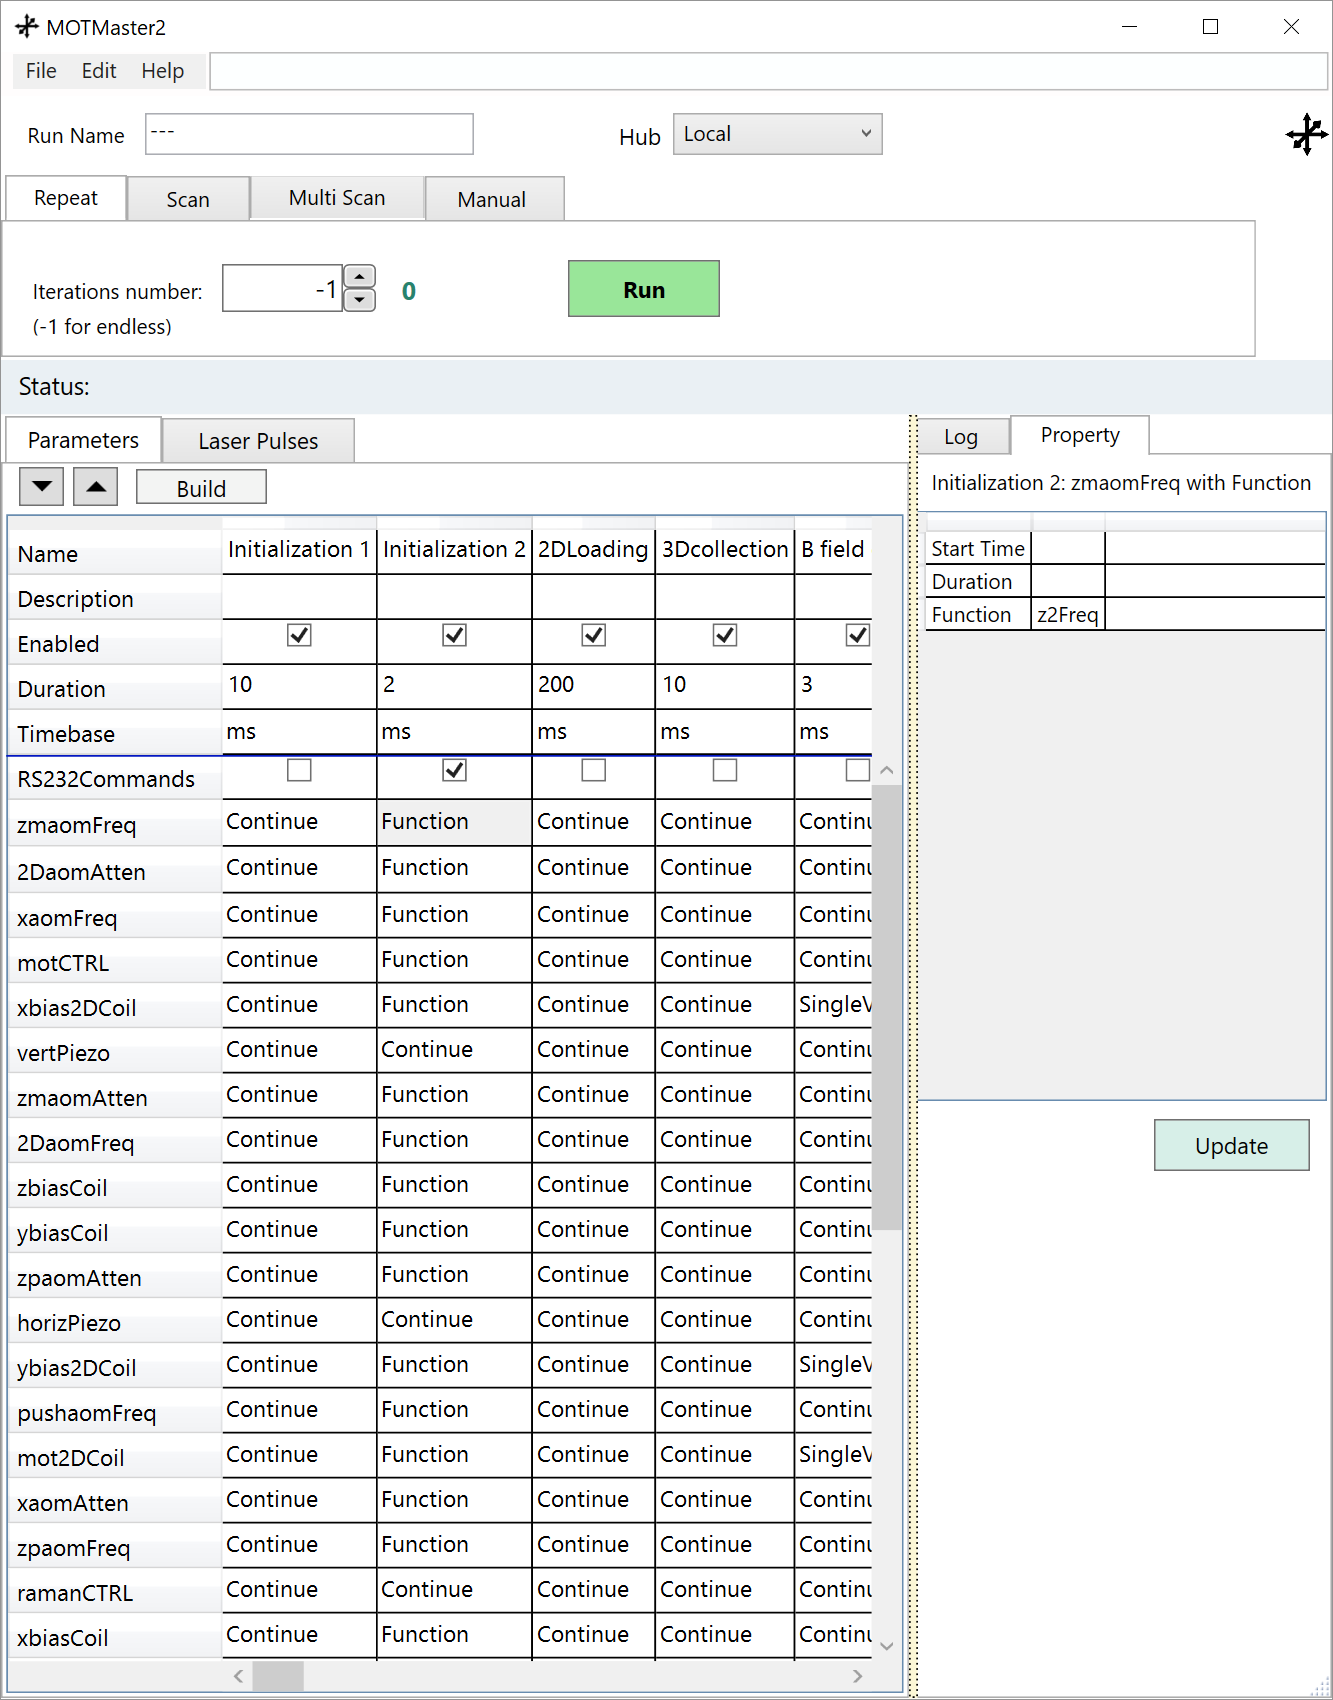
\includegraphics{motmaster_sequence.png}}
    \caption[MOTMaster user interface]{A sequence as represented in the MOTMaster user interface. Each step defines a duration and properties for each output channel. The sequence can either be run repeatedly, or configured to iterate through values of a chosen parameter.}
    \label{fig:motmaster_sequence}
\end{figure}
\par\noindent
After the sequence has finished, any acquired data from the analogue input channels is
streamed to the computer. The data per channel are segmented into arrays that
were acquired during each sequence step, before additional post-processing if
required. Finally, the hardware is reset to its initial state, before
starting the next experiment cycle.

\section{Experiment Control Hardware}\label{sec:mm_control_hardware}
In the preceding sections, the discussion of MOTMaster has been presented
without referring to specific hardware used in this experiment. Subsequent
chapters will introduce components of the experiment that are controlled by a
computer, but it is worth introducing the hardware used to implement this
control. A diagram of the control hardware is shown in~\FigureRef{fig:control_hardware}. All of the \ac{daq} cards are housed on a PXIe-1073 chassis, so that
timing signals such as start triggers and sample clocks can be shared on the
PXI backplane. The analogue output signals are generated on a
PXI-6723 card. This contains 32 analogue output channels and the output of
each is generated using a 13 bit \ac{dac}. Over the maximum voltage range of
\(\pm \sivalue{10}{\volt}\), this corresponds to an output quantisation of
\sivalue{2.44}{\milli\volt}, which did not limit the precision of any
analogue control in the experiment. The analogue output pattern is sampled at
a frequency of \sivalue{100}{\kilo\hertz}, which gives a minimum resolution
of \sivalue{10}{\micro\second}. Any jitter on this sample clock did not
produce any noticeable effects during the experiment. \par\noindent
Two cards on the chassis are able to acquire data from analogue inputs. The
first is a PXIe-6341, which has 16 input channels, each with a 16-bit
\ac{adc}. In addition to this, a counter channel on this card was used to trigger the output of serial messages. During the preliminary stages of the experiment, this bit-depth was
sufficiently large to prevent quantisation effects becoming significant. However
the AI-Q-2010 MEMS accelerometer used in the experiment, discussed further in \SectionRef{subsec:raman_mems}, has an equivalent voltage noise below this quantisation level. Therefore, a
PXI-4462 card, which contains 4 24-bit analogue input channels, was added.
This card is used to acquire data from devices where the higher voltage
resolution is desirable --- namely, the MEMS accelerometer and the
photodiode used to detect the population of atoms in each state after interference.\par\noindent
Digital output signals are generated using a PXI-6541 card. Unlike the
others, this card is controlled using the NI-HSDIO driver. With a maximum
sampling frequency of \sivalue{50}{\mega\hertz}, this card is capable of
generating digital signals at a much higher rate than the PXIe-6341, which
also contains digital output channels. However, the PXIe-6341 card only
contains 8 digital channels that can be timed using a hardware clock, fewer
than required to control the entire experiment.
\par\noindent
Two components of the experiment are controlled during the experiment using
serial communication. The first of these is an interface to the \ac{dds} on
the \Muquans\ laser which control the frequency of the cooling and repump
lasers and is controlled in real-time during the experiment. This
communication protocol is described in further detail in
\SectionRef{subsec:muquans_comm}. Finally, MOTMaster is configured to remotely connect to the M
Squared laser, so that it can control all the parameters necessary to drive
Raman transitions during the experiment. This is done by sending structured
JSON messages that contain commands to implement this control. More detail on how this is used in the experiment is given in
\SectionRef{subsuc:msquared_comm}.
\begin{figure}[!htbp]
    \centering
    \fontsize{16pt}{14pt}
    \resizebox{1\textwidth}{!}{\input{control_hardware.pdf_tex}}
    \caption[Control hardware schematic diagram]{Schematic diagram of the control hardware. The PXIe chassis contains the DAQ cards which generate the analogue and digital waveforms used to control other devices. Signals are routed between the cards to synchronise their operation. Serial communication to the \Muquans laser (\SectionRef{sec:muquans_light}), the M-Squared laser (\SectionRef{sec:msquared_laser})and the CCD camera (\SectionRef{sec:imaging}) are used for their control.}
    \label{fig:control_hardware}
\end{figure}

\section{Experimental Sequence Overview}
The experiment can be broken down into the following stages:
\begin{itemize}
    \item \underline{Loading}: Atoms are loaded from the 2D \ac{mot} into the 3D \ac{mot}.
    \item \underline{Molasses}: Atoms are released from the trap and cooled further in an optical molasses.
    \item \underline{State Preparation}: A sequence of optical and microwave pulses are used to prepare atoms with a narrow velocity spread in the \(\ket{1,0}\) state.
    \item \underline{Interferometry}: A \(\pi/2 - \pi - \pi/2\) sequence of laser pulses drive Raman transitions between the atoms.
    \item \underline{Dectection}: Two laser pulses are used to measure the number of atoms in \(\ket{F=2}\) and the total number, respectively. From these measurements, the interferometer phase difference can be inferred.
\end{itemize}
